\documentclass{article}
\usepackage[utf8]{inputenc}

\usepackage[T2A]{fontenc}
\usepackage[utf8]{inputenc}
\usepackage[polutonikogreek, english,russian]{babel}
\usepackage{csquotes}

\usepackage{hyperref}
\hypersetup{
    colorlinks, citecolor=black, filecolor=black, linkcolor=black, urlcolor=black
}

\usepackage{graphicx}
\graphicspath{ {./images/} }

\newtheorem{definition}{Определение}

\title{Философия}
\author{Лисид Лаконский}
\date{December 2022}

\begin{document}

\maketitle
\tableofcontents
\pagebreak

\section{Философия - 13.12.2022}

\subsection{З. Фрейд: структура личности, бессознательное}

\subsubsection{Структура личности}

\begin{flushleft}

Зигмунд Фрейд утверждал, что личность состоит из трех \textbf{основных элементов}: \textbf{ид}, \textbf{эго} и \textbf{суперэго}

\paragraph{Ид} От латинского "оно", по Фрейду - \textbf{примитивные, инстинктивные и врожденные} аспекты личности.

Полностью функционирует в \textbf{бессознательном} и тесно связан с \textbf{первичными потребностями} (напр. еда, сон, дефекация).

Согласно Фрейду, ид - нечто \textbf{темное, биологическое, хаотичное}, не подчиняющееся никаким правилам. Ид - \textbf{старейшая} структура психики; выражает первичный принцип человеческой жизни - немедленный \textbf{выплеск психической энергии}, производимой биологически обусловленными побуждениями. Немедленная разрядка напряжения получила название \textbf{принцип удовольствия}. Ид следует из этого принципа, выражая себя в \textbf{импульсивной, себялюбивой манере}, не обращая внимания на последствия для других и вопреки самосохранению.

\hfill

Фрейд описал два механизма, посредством которых ид \textbf{избавляет личность от напряжения}:

\begin{enumerate}
    \item Рефлекторные действия - \textbf{автоматически отвечает на сигналы} и, таким образом, сразу снимает напряжение
    \item Первичные процессы представления - вступает в действие тогда, когда рефлекторное действие не может снизить напряжение - \textbf{формирует психический образ объекта}, первично связанного с удовлетворением основной потребности (в примере с голодным ребенком данный процесс может вызвать образ материнской груди или бутылочки молока)
\end{enumerate}

Первичные процессы — нелогичная, \textbf{иррациональная и фантазийная форма человеческих представлений}, характеризующаяся \textbf{неспособностью подавлять импульсы и различать реальное и нереальное}. Поэтому, утверждал Фрейд, для младенца является невыполнимой задача научиться откладывать удовлетворение своих первичных потребностей. Способность к отсроченному удовлетворению впервые возникает, когда маленькие дети понимают, что, помимо их собственных нужд и желаний, есть еще и внешний мир. С появлением этого знания возникает вторая структура личности, \textbf{эго}.

\paragraph{Эго} От латинского "я", по Фрейду это компонент, ответственный за \textbf{принятие решений}. Эго \textbf{стремится выразить и удовлетворить желания ид} в соответствии с ограничениями, налагаемыми внешним миром. Эго получает свою структуру и функцию от ид, эволюционирует из него и заимствует часть энергии ид для своих нужд, чтобы отвечать требованиям социальной реальности. Таким образом, эго помогает \textbf{обеспечить безопасность и самосохранение организма}. Эго использует \textbf{когнитивные и перцептивные процессы} в своем стремлении удовлетворять желания и потребности ид. В отличии от ид, природа которого выражается в поиске удовольствия, эго \textbf{подчиняется принципу реальности}, цель которого — сохранение целостности организма путем отсрочки удовлетворения инстинктов до того момента, когда будет найдена возможность достичь разрядки подходящим способом или будут найдены соответствующие условия во внешней среде.

\paragraph{Суперэго}

Для того, чтобы человек эффективно функционировал в обществе, он должен иметь \textbf{систему ценностей, норм и этики}, разумно совместимых с теми, что приняты в его окружении. Все это приобретается в процессе “социализации”; на языке структурной модели психоанализа — посредством формирования \textbf{суперэго}.

Суперэго \textbf{последний компонент} развивающейся личности. С точки зрения Фрейда, организм не рождается с суперэго, а \textbf{приобретает его благодаря взаимодействию} “формирующими” фигурами (родителями, учителями и т.д.). Суперэго \textbf{является следствием продолжительной зависимости} ребенка от родителей. Оно начинает проявляться, когда ребенок начинает различать “правильно” и “неправильно”.

Фрейд разделил суперэго на \textbf{две подсистемы}:

\begin{enumerate}
    \item Совесть - приобретается \textbf{посредством родительских наказаний} - связана с поступками, за которые \textbf{ребенок получает выговор} - включает в себя \textbf{способность к критической самооценке, наличие моральных запретов и возникновение чувства вины}
    \item Эго-идеал - \textbf{поощрительный аспект}, формируется из того, что \textbf{значимые люди одобряют} или высоко ценят - и, если цель достигнута, \textbf{вызывает чувство самоуважения и гордости}
\end{enumerate}

Суперэго считается полностью сформированным, когда \textbf{родительский контроль сменяется самоконтролем}. Суперэго, пытаясь полностью затормозить любые общественно осуждаемые импульсы со стороны ид, \textbf{пытается направлять человека к абсолютному совершенству} в мыслях, словах и поступках. То есть, оно \textbf{пытается убедить} эго в \textbf{преимуществе идеалистических целей над реалистичными}.

\end{flushleft}

\subsubsection{Бессознательное}

\begin{flushleft}

Фрейд считал, что \textbf{самая глубинная и значимая} область человеческого разума – это \textbf{бессознательное}. Бессознательное является \textbf{хранилищем для примитивных инстинктов, эмоций и воспоминаний}, настолько \textbf{угрожающих сознанию}, что они вытеснены в область бессознательного. Эти подавленные инстинкты и эмоции \textbf{определяют наше повседневное существование}.

\hfill

Фрейду психика человека представляется как \textbf{противостоящие друг
другу сферы сознательного и бессознательного}, представляющие собой существенные характеристики личности. Но обе эти сферы в его структуре представлены неравнозначно: \textbf{бессознательное он считал центральным компонентом}, а \textbf{сознательное – лишь инстанцией}, стоящей над бессознательным и появившейся из него в процессе эволюции психики.

\hfill

По Фрейду человеческая психика делится на \textbf{три области: сознательное, бессознательное и предсознательное}. Эти три сферы психического находятся в состоянии \textbf{постоянного взаимодействия}, а две первых – и в состоянии \textbf{постоянной борьбы} между собой. Каждый поступок человека нужно рассматривать как \textbf{результат борьбы сознательного с бессознательным}.

\paragraph{Формирование бессознательного: вытеснение, влечение}

\textbf{Вытеснение} (подавление, репрессия) — один из механизмов \textbf{психологической защиты} в психодинамическом направлении психологии. Заключается в \textbf{активном, мотивированном устранении чего-либо из сознания}. Обычно проявляется в виде \textbf{немотивированного забывания или игнорирования}.

Как защитный механизм, вытеснение направлено на минимизацию отрицательных переживаний за счёт удаления из сознания того, что эти переживания вызывает. Удалённые из сознания, эти элементы, однако, \textbf{не пропадают из памяти} и \textbf{не перестают влиять на поведение человека и его сны}. Первым вытеснение описал Зигмунд Фрейд, считавший его \textbf{основным механизмом формирования бессознательного}. По его словам, «…судьба \textbf{импульса влечения} может быть определена так, что он наталкивается на сопротивление, которое хочет сделать его недейственным. Тогда при определённых условиях он приходит в \textbf{состояние вытеснения}».

\hfill

\textbf{Влечение} - самовпечатляемость, при которой невозможно уйти или спрятаться от себя поскольку \textbf{неизбежно создается состояние внутреннего дискомфорта и тяжести}. Все влечения Фрейд разделяет на \textbf{две группы}:

\begin{enumerate}
    \item Влечение к жизни (эрос)
    \item Влечение к смерти (танатос)
\end{enumerate}

В мире бессознательного находится \textbf{все то, что хотел бы сделать организм, не будь он связан принципом реальности и культурой}.

\end{flushleft}

\pagebreak
\subsection{К. Юнг: коллективное бессознательное, архетипы}

\subsubsection{Коллективное бессознательное}

\begin{flushleft}

\textbf{Коллективное бессознательное} - особый класс психических явлений, которые в отличие от индивидуального (личного) бессознательного являются \textbf{носителями опыта филогенетического развития человечества, передающегося по наследству через мозговые структуры}. Содержанием коллективного бессознательного, по Юнгу, выступают \textbf{архетипы - всеобщие априорные схемы поведения, которые в реальной жизни человека наполняются конкретным содержанием}.

\hfill

По мнению Юнга, \textbf{существует не только бессознательное субъекта}, но и \textbf{семейное, родовое, национальное, расовое и коллективное бессознательное}. Коллективное бессознательное несет в себе информацию психического мира всего общества, в то время как индивидуальное — информацию психического мира конкретного человека. В отличие от психоанализа, юнгианство рассматривает бессознательное как \textbf{совокупность статичных паттернов, образцов поведения}, которые \textbf{являются врожденными} и лишь нуждаются в актуализации. Так же бессознательное делится на латентные, временно неосознаваемые и подавленные, вытесненные за границы сознания процессы и состояния психики.

\end{flushleft}

\subsubsection{Архетипы}

\begin{flushleft}

\textbf{Архетип} - вид, способ, с которым бессознательное действует на сознание - \textbf{первичный образы}, существовавшие с незапамятных времен, но лишенные ясного содержания.

\hfill

Эти "виды действия" (паттерны) \textbf{происходят от инстинктов и заложены в природе человека}. При рождении у него уже есть в потенциале все архетипы, поэтому и говорится о коллективном бессознательном - совокупности архетипов. Так как архетипы - бессознательны, то \textbf{влияние архетипа сознанием полностью не осознается и поэтому проецируется вовне} (все бессознательное проецируется, и все, что проецируется - бессознательно) и сопровождается эмоциями.

\hfill

При осознании "охваченности" архетипом - \textbf{его влияние сходит на нет и ассимилируется} сознанием. При неосознании архетипа его \textbf{воздействие продолжается}, пока не "застывает" в Персоне - очередной маске эго-сознания. Сами \textbf{архетипы - суть формы, паттерны} и наполняются конкретным личным содержанием только при воздействии на определенное сознание. Поэтому и говорится, что наследуются не "архетипические представления", а именно \textbf{паттерны - пустые формы, сам вид, форма воздействия}. Образы, в которые проецируются архетипы, называются архетипическими представлениями, архетипическими образами и т.д.

\hfill

Специфическое содержание архетипов как реализованных образов \textbf{обеспечивается материалом сознательного опыта}. Таким образом, архетип как таковой — это пустая форма, которая \textbf{должна выводиться или извлекаться} посредством абстракции из класса известных по опыту образов или символов.

\hfill

\textbf{Эго} – центральный архетип в сфере сознания.

\textbf{Персона} – архетип, который показывает \textbf{компромисс между индивидом и обществом}, это маска, которую человек надевает при встречах с другими. Персона – \textbf{внешнее выражение социальности}, она дает возможность, с одной стороны, \textbf{производить определенное впечатление} на людей, а с другой – \textbf{скрыть свою истинную природу, свою индивидуальность}.

\textbf{Тень} – центральный архетип в сфере бессознательного, в котором \textbf{сосредоточена негативная сторона человека}. Тень – это все \textbf{низменное, примитивное}, подспудно дремлющее в глубинах человеческого существа и скрывающееся за масками благопристойности.

\textbf{Анима и Анимус} – архетипы женского и мужского начала, содержащиеся в образах человеческого "Я" и символизирующие собой противоположный пол.

Самость – центральный архетип целостности личности, который \textbf{интегрирует сознательное и бессознательное} в психике человека. Под самостью Юнг понимает \textbf{и подлинный субъект, и целостную личность, и цель жизни человека}.

\hfill

Упомянутые архетипы, как правило, \textbf{воспринимаются в персонифицированной форме}. Они могут появляться как персонажи сновидений и служат источником таких культурных символов, как \textbf{боги и богини}. Они также широко входят в межличностный опыт, часто проецируясь на других людей. Каждый \textbf{архетип может выражаться в большом разнообразии персонификаций}. Конкретный образ анимы \textbf{может быть положительным или отрицательным} и подчеркивать любые качества из допустимого их множества. Другие архетипы, которые Юнг называет \textbf{архетипами трансформации}, не появляются в персональной форме. Они проявляются во многих ситуациях, местах, орудиях, событиях наших сновидений, определяя соответствующие мотивы фольклора. Юнг полагал, что ему удалось идентифицировать наиболее важные архетипы, но нельзя исключить, что \textbf{общее их число бесконечно}, и составить их полный список невозможно.
    
\end{flushleft}

\pagebreak
\subsection{Э. Фромм: социальная психология}

\subsubsection{Социальная психология}

\begin{flushleft}

\textbf{Социальное окружение} для Эриха Фромма (1900-1980) являлось не просто условием, но \textbf{важнейшей детерминантой} развития личности. В отличие от Адлера, Фромм под средой понимал \textbf{не только ближайшее окружение человека, его семью и близких, но и устройство общества}, в котором он живет. Фромм подчеркивал, что наибольшее значение для него имели идеи \textbf{Маркса и Фрейда}, которые он хотел объединить в своей теории. Если от Фрейда он взял \textbf{идею о доминирующей роли бессознательного в личности человека}, то от Маркса — мысль о \textbf{значении социальной формации для развития психики}, а также \textbf{идею о развитии отчуждения при капитализме}.

\hfill

Фромм полагал, что \textbf{движущими силами развития личности} являются две врожденные бессознательные потребности: 

\begin{enumerate}
\item \textbf{потребность в укоренении} - заставляет человека \textbf{стремиться к обществу}, соотносить себя с другими его членами, \textbf{стремиться к общей с ними системе идеалов} и т. п.
\item \textbf{потребность в индивидуализации} толкает к \textbf{изоляции от других, к свободе от давления общества}. 
\end{enumerate}

Эти две потребности являются \textbf{причиной внутренних противоречий и конфликта мотивов}. Стремление примирить эти потребности является \textbf{двигателем не только развития личности, но и общества в целом}.

\hfill

\textbf{Индивидуализация} развивается в ущерб \textbf{укорененности}, от которой человек начинает тосковать, стремясь убежать от обретенной свободы. Это бегство от свободы, характерное для общества, где все друг другу чужие, проявляется не только в желании получить надежную работу, но и в идентификации. В стремлении к индивидуализации люди обычно стремятся к \textbf{«свободе от» других}, от обязательств и догм, определяющих их жизнь в обществе. Желание свободы от всех и любой ценой \textbf{не дает человеку возможности задуматься над тем, зачем ему нужна эта свобода}. Поэтому, обретая ее, он \textbf{не знает, что с ней делать}, и у него возникает \textbf{желание променять ее опять на укорененность}.

\hfill

В то же время есть и другая свобода, \textbf{«Свобода для», необходимая для осуществления наших намерений}. Такая свобода требует \textbf{освобождения} не от всех связей, а \textbf{только от тех, которые мешают в осуществлении задуманного}. Поэтому обретение такой свободы и индивидуальности \textbf{не тяготит человека}, но, наоборот, \textbf{принимается им с радостью}. Именно такая свобода, свобода для жизни с близкими людьми, и \textbf{рождается в любви}. Поэтому Фромм говорил о необходимости построить \textbf{новое общество — «гуманистический идеализм», основанный на любви}.

\hfill

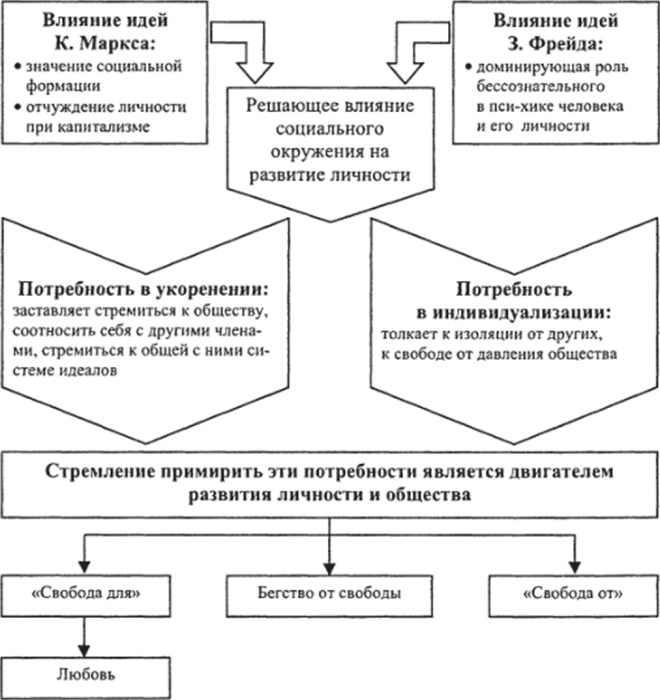
\includegraphics[width=\textwidth]{erich_fromm}

\end{flushleft}

\pagebreak
\subsection{Список литературы}

\subsubsection{Рекомендумая литература}

\begin{enumerate}
    \item Васильев В.В., Кротов А.А., Бугай Д.В. История философии. М.: Академический проспект, 2008
\end{enumerate}

\subsubsection{Дополнительная литература}

\begin{enumerate}
    \item Гуревич П.С. Психоанализ. Т. 1. Фрейдизм и неофрейдизм. М.: Издательство Юрайт, 2019
\end{enumerate}

\end{document}